\chapter{Descriptive overview of Edit Filters on the English Wikipedia}
\label{chap:overview-en-wiki}

The purpose of this chapter (syn?) is to explore the edit filters on the Englisch Wikipedia.
We want to gather a understanding of what types of tasks these filters take over,
and, as far as feasible, trace how these tasks have evolved over time.

%TODO describe what each section is about
The data upon which the analysis is based is described in section~\ref{sec:overview-data}
and the methods we use–in chapter 3.
Section~\ref{sec:patterns} explores (syn) some patterns in the edit filters' usage and..
And we look into the manual classification of EN Wikipedia's edit filters I've undertaken in an attempt to understand what is it that they actually filter in section~\ref{sec:manual-classification}.

%TODO tell a story with the chapter: what do filters do? How have their tasks evolved over time (if feasible) --> maybe tell it along the peak: it is an extraordinary situation, where we can see it is exactly X and Y and Z what filters do

%TODO check whether to discuss this bunch of random questions and where
\begin{comment}
    \item how often were filters with different actions triggered? (afl\_actions) (over time) --> abuse\_filter\_log
    \item what types of users trigger the filters (IPs? registered?) : IPs: 16,489,266, logged in users: 6,984,897 (Stand 15.03.2019);
    \item on what articles filters get triggered most frequently (afl\_title)
    \item what types of user actions trigger filters most frequently? (afl\_action) (edit, delete, createaccount, move, upload, autocreateaccount, stashupload)
    \item in which namespaces get filters triggered most frequently?
    %TODO categorise filters according to which name spaces they apply to; pay special attention to edits in user/talks name spaces (may be indication of filtering harassment) -- check notebook
\end{comment}


\section{Data}
\label{sec:overview-data}

The main part of the present analysis rests upon/is based upon/is grounded in/foundations lie the \emph{abuse\_filter} table from \emph{enwiki\_p}(the database which stores data for the EN Wikipedia), or more specifically a snapshot thereof which was downloaded on January 6th, 2019 via quarry, a web-based service offered by Wikimedia for running SQL queries against their public databases~\footnote{\url{https://quarry.wmflabs.org/}}.
The complete dataset can be found in the repository for the present paper~\cite{github}. % TODO add a more specific link

This table, along with \emph{abuse\_filter\_actions}, \emph{abuse\_filter\_log}, and \emph{abuse\_filter\_history}, are created and used by the AbuseFilter MediaWiki extension~\cite{gerrit-abusefilter-tables}, as discussed in section~\ref{sec:mediawiki-ext}.
Selected queries have been run via quarry against the \emph{abuse\_filter\_log} table as well.
Unfortunately, the \emph{abuse\_filter\_history} table which will be necessary for a complete historical analysis of the edit filters is currently not exposed to the public due to security/privacy concerns~\cite{phabricator}.
Therefore, the present work only touches upon historical trends in a qualitative fashion. %TODO how are these determined: API to abuse_filter_history; general stats from abuse_filter
or qualitatively shows patterns.
A comprehensive historical analysis is therefore (syn!) one of the possibilities/directions for future studies (syn) discussed in section~\ref{sec:further-studies}.

%TODO maybe move to appendix; mention tables have been discussed in~\ref{sec:mediawiki-ext} and only quote here the one for abuse\_filter since we are using the data
A concise description of the tables has been offered in section~\ref{sec:mediawiki-ext} which discusses the AbuseFilter MediaWiki extension in more detail.
Here, only the schema of the \emph{abuse\_filter} table has been included (figure~\ref{fig:db-schemas-af}), since that is the data the majority of the present analysis is based upon.
For further reference, the schemas of all four tables can be viewed in figures~\ref{fig:app-db-schemas-af},~\ref{fig:app-db-schemas-afl},~\ref{fig:app-db-schemas-afh} and~\ref{fig:app-db-schemas-afa} in the appendix.

%TODO incorporate this
and, of course, the whole \emph{abuse\_filter} table snapshot can be consulted in the repository~\cite{github}.

\begin{figure*}
\begin{verbatim}
abuse_filter
+--------------------+----------------+------+-----+---------+----------------+
| Field              | Type           | Null | Key | Default | Extra          |
+--------------------+----------------+------+-----+---------+----------------+
| af_id              | bigint(20)     | NO   | PRI | NULL    | auto_increment |
| af_pattern         | blob           | NO   |     | NULL    |                |
| af_user            | bigint(20)     | NO   | MUL | NULL    |                |
| af_user_text       | varbinary(255) | NO   |     | NULL    |                |
| af_timestamp       | binary(14)     | NO   |     | NULL    |                |
| af_enabled         | tinyint(1)     | NO   |     | 1       |                |
| af_comments        | blob           | YES  |     | NULL    |                |
| af_public_comments | tinyblob       | YES  |     | NULL    |                |
| af_hidden          | tinyint(1)     | NO   |     | 0       |                |
| af_hit_count       | bigint(20)     | NO   |     | 0       |                |
| af_throttled       | tinyint(1)     | NO   |     | 0       |                |
| af_deleted         | tinyint(1)     | NO   |     | 0       |                |
| af_actions         | varbinary(255) | NO   |     |         |                |
| af_global          | tinyint(1)     | NO   |     | 0       |                |
| af_group           | varbinary(64)  | NO   | MUL | default |                |
+--------------------+----------------+------+-----+---------+----------------+
\end{verbatim}
  \caption{abuse\_filter schema}~\label{fig:db-schemas-af}
\end{figure*}

\section{Descriptive statistics/Patterns/General traits of the filters}
\label{sec:patterns}

In this section, we explore some general traits/patterns of/trends in the edit filters on Engish Wikipedia, or respectively the data from the \emph{abuse\_filter} table.
The scripts that generate the statistics (syn?) discussed here, can be found in the jupyter notebook in the project's repository. %TODO add link after repository has been cleaned up

\subsection{Filter characteristics}
% General stats
As of January 6th, 2019 there are $954$ filters in the \emph{abuse\_filter} table.
It should be noted, that if a filter gets deleted, merely a flag is set to indicate so, but no entries are removed from the database.
So, the above mentioned $954$ filters are all filters ever made up to this date.
This doesn't mean that it never changed what the single filters are doing, since edit filter managers can freely modify filter patterns, so at some point the filter could be doing one thing and in the next moment it can be filtering a completely different phenomenon.
There are cases of filters being ``repurposed'' or modified to filter for example a more general occurance/phenomenon.
This doesn't happen very often though.
$361$ of all filters are public, the remaining $593$–hidden.
$110$ of the public ones are active, $35$ are disabled, but not marked as deleted, and $216$ are flagged as deleted.
Out of the $593$ hidden filters $91$ are active, $118$ are disabled (not deleted), and $384$ are deleted.
The relative proportion of these groups to each other can be viewed on figure~\ref{fig:general-stats}.

\begin{figure}
\centering
  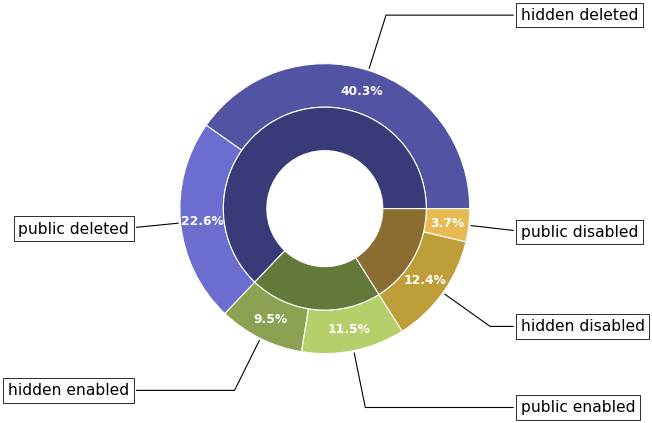
\includegraphics[width=0.9\columnwidth]{pics/general-stats-donut.png}
  \caption{There are 954 edit filters on EN Wikipedia}~\label{fig:general-stats}
\end{figure}

\subsection{Filter actions}
An interesting parameter we could observe are the currently configured filter actions for each filter.
Figure~\ref{fig:all-active-filters-actions} depicts the frequency of signle actions for all enabled filters (note some filters have multiple actions enabled).
And figures~\ref{fig:active-public-actions} and~\ref{fig:active-hidden-actions} show the actions of all enabled public and hidden filters respectively.
It is noticeable that the most common action for the enabled hidden filters is ``disallow'' whereas most enabled public filters are set to ``tag'' or ``tag,warn''.
This coincides/is congruent with the community's claim that hidden filters target particularly perstistent vandalism, which is best outright disallowed.
Most public filters on the other hand still assume good faith from the editors and try to dissuade them from engaging in disruptive behaviour by using warnings or just tag conspicious behaviour for further investigation.

\begin{figure}
\centering
  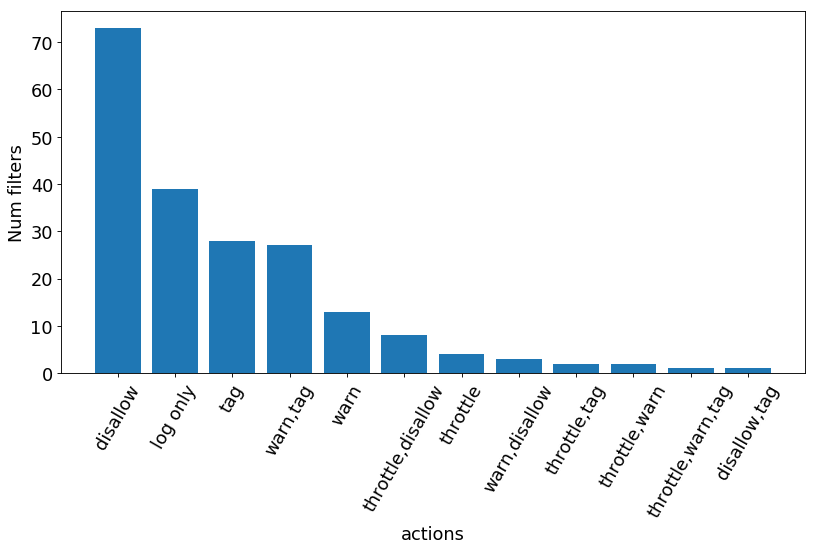
\includegraphics[width=0.9\columnwidth]{pics/all-active-filters-actions.png}
  \caption{EN Wikipedia edit filters: Filters actions for all filters}~\label{fig:all-active-filters-actions}
\end{figure}

%\begin{figure}
%\centering
%  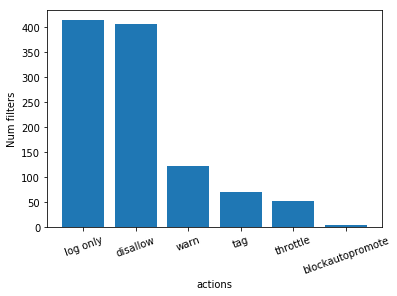
\includegraphics[width=0.9\columnwidth]{pics/all-filters-actions.png}
%  \caption{EN Wikipedia edit filters: Filters actions for all filters}~\label{fig:all-filters-actions}
%\end{figure}

\begin{figure}
\centering
  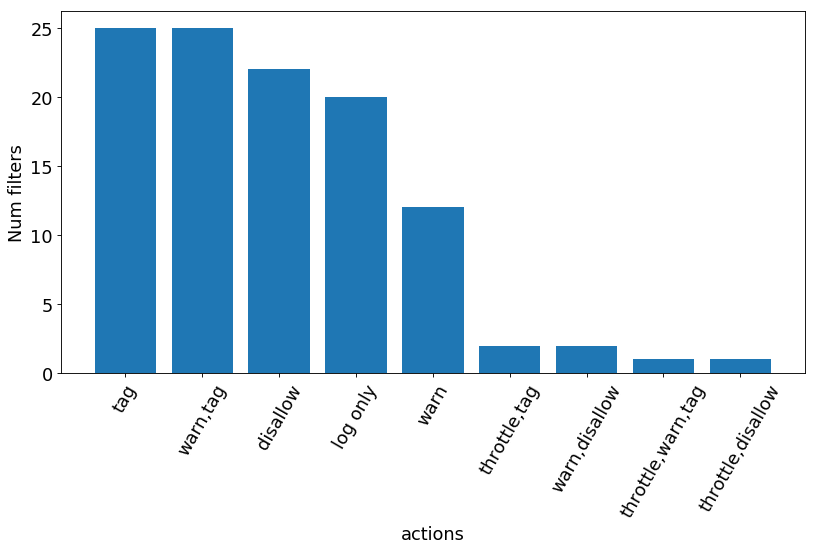
\includegraphics[width=0.9\columnwidth]{pics/active-public-actions-big.png}
  \caption{EN Wikipedia edit filters: Filters actions for enabled public filters}~\label{fig:active-public-actions}
\end{figure}

\begin{figure}
\centering
  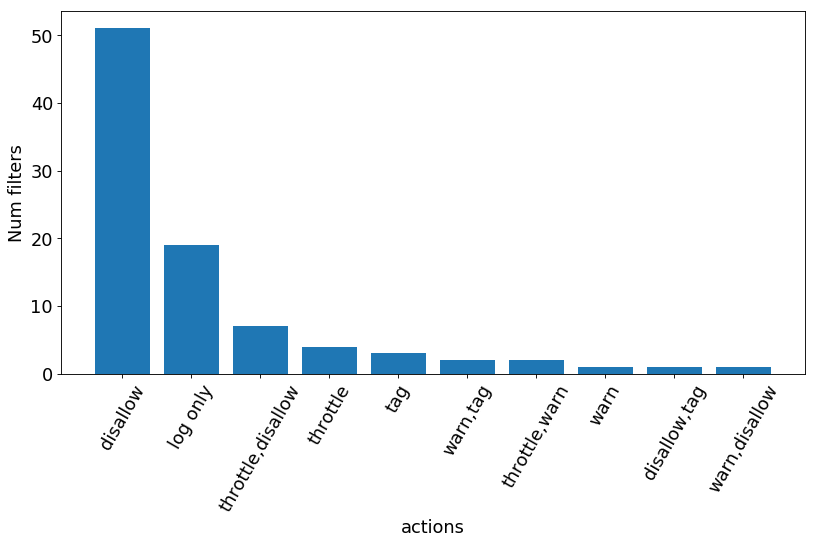
\includegraphics[width=0.9\columnwidth]{pics/active-hidden-actions-big.png}
  \caption{EN Wikipedia edit filters: Filters actions for enabled hidden filters}~\label{fig:active-hidden-actions}
\end{figure}

\subsection{What do filters target}%: general behaviour vs edits by single users

Most of the public filters target disruptive behaviours in general (e.g. filter 384 disallows ``Addition of bad words or other vandalism'' by any non-confirmed user).
There are however some which target particular users or particular pages.
Arguably, (see guidelines) an edit filter may not be the ideal mechanism for this latter purpose, since every incoming edit is checked against all active filters.
In addition, time and again various filters have been introduced to track some specific sort of behaviour which was however neither malicious nor disruptive.
This contradicts/defies/fails the purpose of the mechanism and thus such filters have been (quite swiftly) disabled.
Some filters target (syn!) insults in general, and there are such which target (syn!) specifically insults aimed at particular persons (often edit filter managers).

A lot of hidden filters target specific users/problems.
\begin{comment}
  ** there are quite some filters targeting particular users: 290 (targets an IP range), 177 ('User:Television Radio'), 663 ('Techno genre warrior
', targets specific IP ranges)
  ** there are also some targetting particular pages (verify!), although this clashed with the guidelines: 264 "Specific-page vandalism" (it's hidden though, so we don't know what exactly it's doing); 401 ("Red hair" vandalism); there's smth with the main page; 715 "IP notification on RFP/C"
  ** there are also filters such as 199 (Unflagged bots) which were implemented in order to track something which was not quite malicious or abusive and were thus deemed inappropriate use of filters by the community and consequently (quite swiftly) deleted
  ** some target insults in general and some contain regexes containing very specifically insults directed towards edit filter managers (see filter 12)
\end{comment}

\subsection{Public and Hidden Filters}

As signaled in section~\ref{section:4-history}, historically it was planed to make all edit filters hidden from the general public.
The community discussions rebutted that so a guideline was drafted calling for
hiding filters ``only where necessary, such as in long-term abuse cases where the targeted user(s) could review a public filter and use that knowledge to circumvent it.''~\cite{Wikipedia:EditFilter}.
This is however not always complied with and edit filter managers do end up hiding filters that target general vandalism despite consensus that these should be public~\cite{Wikipedia:PrivacyGeneralVandalism}.
Such cases are usually made public eventually (examples hereof are filters 225 ``Vandalism in all caps'', 260 ``Common vandal phrases'', or 12 ``Replacing a page with obscenities'').
Also, oftentimes when a hidden filter is marked as ``deleted'', it is made public. %TODO examples?

Still, it draws attention that currently nearly $2/3$ of all edit filters are not viewable by the general public (compare figure~\ref{fig:general-stats}).
Unfortunately, without the full \emph{abuse\_filter\_history} table we cannot know how this ration has developed historically.
However, the numbers fit the assertion of the extension's core developer according to whom edit filters target particularly determined vandals.

On the other hand, if we look at the enabled filters only, there are actually more or less the same number of public enabled and hidden enabled filters ($110$ vs $91$).
This leads us to the hypothesis that it is rather that hidden filters have higher fluctuation rates, i.e. that they target specific phenomena that are over after a particular period of time after which the filters get disabled and eventually–deleted.
This makes sense when we compare it to the hidden vs public filter policy: hidden filters for particular cases and very determined vandals, public filters for general patterns.

%TODO check hits: public vs hidden

%TODO this seems out of place
Further, caution in filter naming is suggested for hidden filters and editors are encouraged to give such filters just simple description of the overall disruptive behaviour rather than naming a specific user that is causing the disruptions.
(The latter is not always complied with, there are indeed filters named after the accounts causing a disruption.)

% TODO this whole paragraph seems redundant with chapter 4
Only edit filter editors (who have the \emph{abusefilter-modify} permission) and editors with the \emph{abusefilter-view-private} permission can view hidden filters.
The latter is given to edit filter helpers–editors interested in helping with edit filters who still do not meet certain criteria in order to be granted the full \emph{abusefilter-modify} permission, editors working with edit filters on other wikis interested in learning from the filter system on English Wikipedia, and Sockpuppet investigation clerks~\cite{Wikipedia:EditFilterHelper}.
As of March 17, 2019, there are 16 edit filter helpers on EN Wikipedia~\footnote{\url{https://en.wikipedia.org/wiki/Special:ListUsers/abusefilter-helper}}.
Also, all administrators are able to view hidden filters.

There is also a designated mailing list for discussing these.
It is specifically indicated that this is the communication channel to be used when dealing with harassment (by means of edit filters)~\cite{Wikipedia:EditFilter}.
Furthermore, it is signaled, that the mailing list is meant for sensitive cases only and all general discussions should be held on-wiki~\cite{Wikipedia:EditFilter}.

\section{Filter activity}

\subsection{Distinct filters over the years + condition limit}
Thanks to quarry, we have all the filters that were triggered from the filter log per year, % I do have the whole table actually, don't I?
from 2009 (when filters were first introduced/the MediaWiki extension was enabled) till end of 2018, with their corresponding number of times being triggered:
Table~\ref{tab:active-filters-count} summarises the numbers of distinct filters that got triggered over the years.
So, the number of distinct filters that have been triggered over the years (syn!) varies between $154$ in year 2014 and $254$ in 2018.
The explanation for this not particularly wide range of active filters lies probably in the so-called condition limit.
According to the edit filters' documentation~\cite{Wikipedia:EditFilterDocumentation}, the condition limit is a hard-coded treshold of total available conditions that can be evaluated by all active filters.
Currently, it is set to $1,000$.
The motivation for the condition limit is to avoid performance issues since every incoming edit is checked against all currently enabled filters which means that the more filters are active the longer the checks take.
However, the page also warns that counting conditions is not the ideal metric of filter performance, since there are simple comparisons that take significantly less time than a check against the \emph{all\_links} variable for example (which needs to query the database)~\cite{Wikipedia:EditFilterDocumentation}.

\begin{table}
  \centering
  \begin{tabular}{l r }
    % \toprule
    Year & Num of distinct filters \\
    \hline
    2009 & 220 \\
    2010 & 163 \\
    2011 & 161 \\
    2012 & 170 \\
    2013 & 178 \\
    2014 & 154 \\
    2015 & 200 \\
    2016 & 204 \\
    2017 & 231 \\
    2018 & 254 \\
    % \bottomrule
  \end{tabular}
  \caption{Count of distinct filters that got triggered each year}~\label{tab:active-filters-count}
\end{table}

\subsection{Most active filters of all times}
The ten most active filters of all times (with number of hits and public description) are displayed in table~\ref{tab:most-active-actions}.
For a more detailed reference, the ten most active filters of each year are listed in the appendix. %TODO are there some historical trends we can read out of it?

Already, a couple of patterns draw attention when we look at the most active (syn!) filters:
They seem to catch a combination of possibly good faith edits which were none the less unconstructive (such as removing references, section blanking or large deletions)
and what the community has come to call ``silly vandalism''~\cite{Wikipedia:VandalismTypes}: repeating characters and inserting profanities.
Interestingly, that's not what the developers of the extension believed it was going to be good for:
``It is not, as some seem to believe, intended to block profanity in articles (that would be extraordinarily dim), nor even to revert page-blankings, '' claimed its core developer on July 9th 2008~\cite{Wikipedia:EditFilterTalkArchive1Clarification}.
Rather, among the 10 most active filters, it is filter 527 ``T34234: log/throttle possible sleeper account creations'' which seems to target what most closely resembles the intended aim of the edit filter extension. %TODO explain again what the intended aim was

Another assumption that proved to be wrong/didn't quite carry into effect was that ``filters in this extension would be triggered fewer times than once every few hours''.
As a matter of fact, a quick glance at the AbuseLog~\footnote{\url{https://en.wikipedia.org/wiki/Special:AbuseLog}} confirms that there are often multiple filter hits per minute.

\begin{table*}
  \centering
    \begin{tabular}{r r p{8cm} p{2cm} }
    % \toprule
        Filter ID & Hitcount & Publicly available description & Actions \\
    \hline
       61 & 1,611,956 & new user removing references & tag \\
      135 & 1,371,361 & repeating characters & tag, warn \\
      527 & 1,241,576 & T34234: log/throttle possible sleeper account creations (hidden filter) & throttle \\
      384 & 1,159,239 & addition of bad words or other vandalism & disallow \\
      172 & 935,925 & section blanking & tag \\
       30 & 840,871 & large deletion from article by new editors & tag, warn \\
      633 & 808,716 & possible canned edit summary & tag \\
      636 & 726,764 & unexplained removal of sourced content & warn \\
        3 & 700,522 & new user blanking articles & tag, warn \\
      650 & 695,601 & creation of a new article without any categories & (log only) \\
  \end{tabular}
  \caption{What do most active filters do?}~\label{tab:most-active-actions}
\end{table*}

\begin{comment}
    \item is it new filters that get triggered most frequently? or are there also very active old ones? -- we have the most active filters per year, where we can observe this. It's a mixture of older and newer filter IDs (they get an incremental ID, so it is somewhat obvious what's older and what's newer); is there a tendency to split and refine older filters?
\end{comment}

% Most active filters per year
%TODO compare with table and with most active filters per year: is it old or new filters that get triggered most often? (I'd say it's a mixture of both and we can now actually answer this question with the history API, it shows us when a filter was first created)

\subsection{Filter hits per month (+peak)}
We can follow/track/backtrack the number of filter hits over the years (syn) on figure~\ref{fig:filter-hits}.
There is a dip in the number of hits in late 2014 and quite a surge in the beginnings of 2016.
Here is the explanation to that:
%TODO discuss peak! (and overall pattern)
\begin{comment}
Looking at january, feb, march 2016 vs sept 2016
- high number of account creation attempts
- a lot of (viagra) spam
- a bunch of very active russian IPs publishing the spam
- the exact moment seems arbitrary


till now it comes to attention that a lot of accounts named something resembling <FirstnameLastname4RandomLetters> were trying to create an account  (while logged in?) (or maybe it was just that the creation of these particular accounts itself was denied); this triggers filter 527 ("T34234: log/throttle possible sleeper account creations
")
There are in the meantime over 5 pages of them, it is definitely happening automatically

TODO: download data; write script to identify actions that triggered the filters (accountcreations? edits?) and what pages were edited
Note: do hidden filters appear in this numbers and in the table? (They are definitely not displayed in the front end of the AbuseLog) -- they do.
\end{comment}

%TODO strectch plot so months are readable; darn. now it's too small on the pdf. Fix it! May be rotate to landscape?
\begin{figure}
\centering
  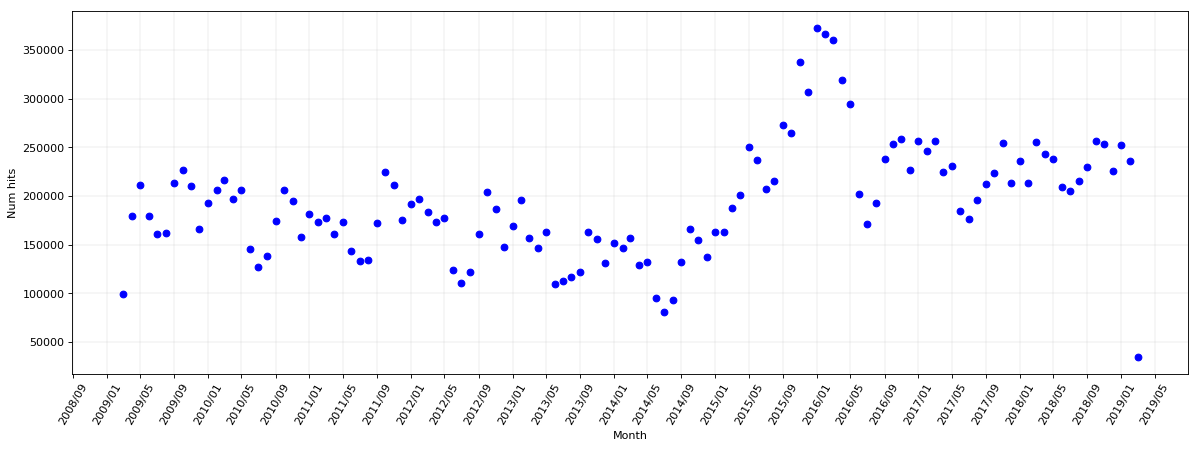
\includegraphics[width=0.9\columnwidth]{pics/filter-hits-zoomed.png}
  \caption{EN Wikipedia edit filters: Number of hits per month}~\label{fig:filter-hits}
\end{figure}


\section{History}

The present section explores qualitatively/highlights patterns in the creation and usage of edit filters.
Unfortunately, no extensive quantitative analysis of these patterns was possible, since for it, an access to the \emph{abuse\_filter\_history} table is needed.
The table is currently not replicated via.. and no public dump is accessible via the toolserver. %TODO elaborate
This seems to have been the case in the past, however, due to security concerns the dumps were discontinued. %TODO cite phabricator
A short term solution to renew the public replicas was not possible, so the present chapter only shows some patterns (syn!) observed via manual browsing of different filters' history via the exposed API endpoint which allows querying the \emph{abuse\_filter\_history} table for public filters.

\subsection{Filter Usage/Activity}

Following general patterns (syn!) of filter usage were observed:
There are filters that have been switched on for a while, then deactivated and never activated again.
Some of them had only been active very briefly before they were switched off and deleted.
There are a couple of different reasons for that:
The filter in question was only testing a pattern which was eventually merged in another filter (e.g.: ). 440 was merged in 345 (or was it a duplicate?)
The edit filter managers decided not to implement the filter, because edit filters were deemed an inappropriate tool to deal with the problem at hand (e.g. ...)308), 199 ('Unflagged Bots');
  ** switched off, bc filter was deemed inappropriate to deal with the issue at hand: 484 "Shutdown of ClueBot by non-admin user" (From the comments: " Just sysop-protect the page if you don't want non-admins messing with it. --Reaper 2012-09-06")
or decides to not implement the thing (that way); 290 (disabled, since relevant pages were protected);
or, because there were hardly any hits, so there wasn't really a problem at all ( 304, 67, 122, 401 ("Red hair" vandalism)). %result of editors implementing a filter "just to see if it catches anything"?
There are also cases in which filter managers implement a filter targeting the same phenomenon in parallel and without knowing of each other.
These duplicate cases (syn!) are also merged eventually, or alternatively all but one of them are switched off: 891 and 893
Sometimes, vandalism trends are only temporary and after a period of activity, the filters become stale.
This is also a reason for filters to be eventually powered off in order to save conditions from the condition limit.
Examples thereof are:302 (switched off on the grounds of insufficient activity),81 (bad charts)
 211 ("Disable, appears to be inactive (log only filter). If you are using this filter, please let me know, and I'll reenable it -Prodego"); 20 ("A waste of processor time, deleted -Prodego"); 663?
There are also filters that were switched off because they weren't doing what they were supposed to and only generated a big amount of false positives: (false positives is a plausible option here): 394,  14 (disabled in couple of hours)

\begin{comment}
%TODO This is a duplicate of a paragraph in 4.5.1. Does it fit better here?
% this actually fits also in the patterns of new filters in chap.5; these are the filters introduced for couple of days/hours, then switched off to never be enabled again
Edit filter managers often introduce filters based on some phenomena they have observed caught by other filters, other algorithmic quality control mechanisms or general experience.
As all newly implemented filters, these are initially enabled in logging only mode until enough log entries are generated to evaluate whether the incident is severe and frequent enough to need a filter.
\end{comment}

Then, there are filters switched on for a while, deactivated for a while and activated again.
Sometimes because a pattern of vandalism is re-occuring, and sometimes–in order to fix technical issues with the filters: 61, 98 (was deactivated briefly since an editor found the "warn" action unfounded; re-enabled to tag), 148 ("20160213 - disabled - possible technical issue - see edit filter noticeboard - xaosflux")

Another group constitute enabled filters that have never been switched off since their introduction.
  11 (verify), 79 (with brief periods of being disabled for couple of minutes/hours, probably in order to update the pattern), 164, 642 (if we ignore the 2min period it was disabled on 13.4.2018), 733 (2.11.2015-present), 29 (18.3.2009-present), 30 (18.3.2009-present), 33 (18.3.2009-present), 39 (18.3.2009-present), 50 (18.3.2009-present), 59 (19.3.2009-present), 80 (22.3.2009-present)
There are also some filters that have always been enabled with the exception of brief periods of time when the filter was deactivated (and the activated again), probably in order to update the conditions: 79, 135 (there were couple of others in Shirik's list, go back and look);
There seems to be a tendency that all actions but logging (which cannot be switched off) are took out, when edit filter managers are updating the regex of the filter.

\subsection{Triggered actions change over time}
%TODO leave this here or move to filter characteristics?
It is not uncommon, that the action(s) a particular filter triggers change over time.
As of the guidelines for implementing new filters, every filter should be enabled in ``log only'' mode at its introduction.
After it has been deemed that the filter actually acts as desired, usually additional actions are switched on~\cite{Wikipedia:EditFilterInstructions}.
Sometimes, when a wave of particularly persistent vandalism arises, a filter is temporarily set to ``warn'' or ``disallow'' and the actions are removed again as soon as the filter is not tripped very frequently anymore. %TODO examples?

\subsection{How do filters emerge?}
  ** an older filter is split? 79 was split out of 61, apparently; 285 is split between "380, 384, 614 and others"; 174 is split from 29
  ** several older filters are merged?
  ** or functionality of an older filter is took and extended in a newer one (479->631); (82->278); (358->633);
  ** new condition(s) are tested and then merged into existing filter : stuff from 292 was merged to 135 (https://en.wikipedia.org/wiki/Special:AbuseFilter/history/135/diff/prev/4408 , also from 366; following the comments from https://en.wikipedia.org/wiki/Special:AbuseFilter/292 it was not conceived as a test filter though, but it was rather merged in 135 post-factum to save conditions); 440 was merged into 345; apparently 912 was merged into 11 (but 11 still looks like checking for "they suck" only^^); in 460: "Merging from 461, 472, 473, 474, and 475. --Reaper 2012-08-17"
  ** an incident caught repeatedly by a filter motivates the creation of a dedicated filter (994)
  ** filter is shut down, because editors notice there are 2 (or more filters) that do nearly identical checks: 344 shut down because of 3

  ** "in addition to filter 148, let's see what we get - Cen" (https://en.wikipedia.org/wiki/Special:AbuseFilter/188) // this illustrates the point that edit filter managers do introduce stuff they feel like introducing just to see if it catches something

\section{People}
\subsection{Filter makers}

Here, a few characteristics of the edit filter managers group are discussed.
As mentioned in section~\ref{}, EN Wikipedia has 154 edit filter managers as of (date).
The group is as discussed (syn!) quite small.
(However, for comparison there are only 4 users in the edit filter managers group on the Catalan Wikipedia and the role does not exist at all on the German, Spanish and Russian ones which leads to the assumption that for these languages all administrators have the \emph{abusefilter\_modify} permission.) %TODO check!

The edit filter managers group is quite stable, with only 4 users who have become an edit filter manager since November 2016 (according to the discusssion archives of the edit filter noticeboard where the permission is requested)~\cite{}.
Since the edit filter helper group has been created in September 2017, only 11 users have been granted the corresponding permissions and only one of them has been subsequently ``promoted'' to become an edit filter manager.
(Interestingly, currently (July 2019) there are 19 people in the edit filter helpers group, so apparently some of them have received the right although no records are there on the noticeboard??)

Moreover, quite some of the 154 edit filter managers on English Wikipedia have a kind of ``not active at the moment'' banner on their user page, which leads to the conclusion that the edit filter managers group is aging.

% Has it been the same people from the very beginning?

% What type of work do the different managers take over?
There are a couple of very active managers who seem to keep an overview over all filters and do maintenance work on them e.g. updating conditions to optimise evaluation or updating (syn!) deprecated variable names upon updates (syn!) of the extension's code.

Further interesting questions come to mind such as whether there are edit filter managers who specialise in creating different types of edit filters (compare manual classification).
However, in order to be able to answer this, an access to the whole \emph{abuse\_filter\_history} table is needed, so this remains a question (syn!) for future inquiry.

\subsection{Who trips filters}

- IPs and (newly) registered users

\begin{comment}
# Memo new users

When comparing the *vandalism* and *good faith* memos, it comes to attention that both type of edits are usually performed by new(ly/recently registered) users (or IP addresses).

A user who just registered an account (or who doesn't even bother to) is most probably inexperienced with Wikipedia, not familiar with all policies and guidelines and perhaps nor with MediaWiki syntax.

It is also quite likely (to be verified against literature!) that majority of vandalism edits come from the same type of newly/recently registered accounts.
In general, it is rather unlikely that an established Wikipedia editor should at once jeopardise the encyclopedia's purpose and start vandalising.
Although apparently there are determined trolls who ``work accounts up'' to admin and then run rampant.
\end{comment}

\section{Types of edit filters: Manual Classification}
\label{sec:manual-classification}

The aim of this section is to get a better understanding of what exactly it is that edit filters are filtering.
Based on the grounded theory methodology presented in chapter~\ref{chap:methods}, I applied emergent coding to all filters, scrutinising their patterns, comments and actions.

Three big clusters of filters were identified, namely ``vandalism'', ``good faith'', and ``maintenance'' (and the auxiliary cluster ``unknown''). %TODO define what each of them are; I actually work with 8 main clusters in the end; Unify this
These are discussed in more detail later in this section.

\subsection{Labeling process and challenges}

As already mentioned, I started coding strongly influenced by the coding methodologies applied by grounded theory scholars (see chapter~\ref{chap:methods}) and let the labels emerge during the process.
I looked through the data paying special attention to the name of the filters (``af\_public\_comments'' field of the \emph{abuse\_filter} table), the comments (``af\_comments''), the regular expression pattern constituting the filter (``af\_pattern''), and the designated filter actions (``af\_actions'').

The assigned codes emerged from the data: some of them being literal quotes of terms used in the decription or comments of a filter, while others summarised the perceived filter functionality.
In addition to that, for vandalism related labels, I used some of the vandalism types identified by the community in~\cite{Wikipedia:VandalismTypes}.
However, this typology was regarded more as an inspiration instead of being adopted 1:1 since some of the types were quite general whereas more specific categories seemed to render more insights.
For instance, I haven't applied the ``addition of text'' category since it seemed more insightful/useful(syn!) to have more specific labels such as ``hoaxing'' or ``silly\_vandalism'' (check the code book in the appendix~\ref{app:code_book} for definitions).
Moreover, I found some of the proposed types redundant.
For example, ``sneaky vandalism'' seems to overlap partially with ``hoaxing'' and partially with ``sockpuppetry'', ``link vandalism'' mostly overlaps with ``spam'' or ``self promotion'' (although not always), and for some reason, ``personal attacks'' are listed twice.

I have labeled the dataset twice.
The motivation therefor was to return to it once I've gained better insight into the data and use this newly gained knowledge to re-evaluate ambiguous cases, i.e. re-label some data with codes that emerged later in the process.
This mode of labeling is congruous with the simultaneous coding and data analysis suggested by grounded theorists (compare section~\ref{sec:gt}).

%1st labeling
Following challenges were encountered during the first round of labeling.
There were some ambiguous cases which I either tagged with the code I deemed most appropriate and a question mark, or assigned all possible labels (or both).
There were also cases for which I could not gather any insight relying on the name, comments and pattern, since the filters were hidden from public view and the name was not descriptive enough.
However, upon some further reflection, I think it is safe to assume that all hidden filters target a form of (more or less grave) vandalism, since the guidelines suggest that filters should not be hidden in the first place unless dealing with cases of persistent and specific vandalism where it could be expected that the vandalising editors will actively look for the filter pattern in their attempts to circumvent the filter\cite{Wikipedia:EditFilter}.
Therefore, during the second round of labeling I tagged all hidden filters for which there weren't any more specific clues (for example in the name of the filter) as ``hidden\_vandalism''.
And then again, there were also cases, not necessarily hidden, where I could not determine any suitable label, since I didn't understand the regex pattern, and/or none of the existing categories seemed to fit, and/or I couldn't think of an insightful new category to assign.
During the first labeling, these were labeled 'unknown', 'unclear' or 'not sure'.
For the second round, I have unified all of them under 'unclear'.

For a number of filters, it was particularly difficult to determine whether they were targeting vandalism or good faith edits.
The only thing that would have distinguished between the two would have been the contributing editor's motivation, which we had no way of knowing.
During the first labeling session, I tended to label such filters with ``vandalism?, good\_faith?''.
For the second labeling, I stuck to the ``assume good faith'' guideline~\cite{Wikipedia:GoodFaith} myself
and only labeled as vandalism cases where good faith was definitely out of the question.
One feature which guided me here was the filter action which represents the judgement of the edit filter manager(s).
Since communication is crucial when assuming good faith, all ambiguous cases which have a less ``grave'' filter action such as ``tag'' or ``warn'' (which seeks to give feedback and thereby effect/influence a constructive contribution) have received a ``good\_faith'' label.
On the other hand, filters set to ``disallow'' were tagged as ``vandalism'' or a particular type thereof, since the filter action is a clear sign that at least the edit filter managers have decided that seeking a dialog with the offending editor is no longer an option. %TODO check whether that's really the case

%TODO compare also with revising codes as the analysis goes along according to Grounded Theory
For the second round of labeling, I tagged the whole dataset again using the compiled code book (see \ref{app:code_book}) and assigned to every filter exactly one label–the one deemed most appropriate (although oftentimes alternative possibilites were listed as notes), without looking at the labels I assigned the first time around.
I intended to compare the labels from both coding sessions and focus on more ambiguous (syn) cases, re-evaluting them using all available information (patterns, public comments, labels from both sessions + any notes I made along the line).
Unfortunately, there was no time, so the analysis of the present section is based upon the second round of labeling.
Comparing codes from both labeling sessions and refining the coding is one of the possibilities for future research. %TODO (re-formulate!)

%TODO disclose links to 1st and 2nd labelling
First round of labeling is available under \url{https://github.com/lusy/wikifilters/blob/master/filter-lists/20190106115600_filters-sorted-by-hits-manual-tags.csv}.

\begin{comment}
% Kept as a possible alternative wording for private vs public and labeling decisions in ambiguous cases
It was not always a straightforward decision to determine what type of edits a certain filter is targeting.
This was of course particularly challenging for private filters where only the public comment (name) of the filter was there to guide the coding.
On the other hand, guidelines state up-front that filters should be hidden only in cases of particularly persistent vandalism, in so far it is probably safe to establish that all hidden filters target some type of vandalism.
However, the classification was difficult for public filters as well, since oftentimes what makes the difference between a good-faith and a vandalism edit is not the content of the edit but the intention of the editor.
While there are cases of juvenile vandalism (putting random swear words in articles) or characters repetiton vandalism which are pretty obvious, that is not the case for sections or articles blanking for example.
For these, from the edit alone there is no way of knowing whether the deletion was malicious or the editor conducting it just wasn't familiar with say the correct procedure for moving an article.
\end{comment}

\begin{comment}
%TODO where to put this?
Users are urged to use the term "vandalism" carefully, since it tends to offend and drive people away.
("When editors are editing in good faith, mislabeling their edits as vandalism makes them less likely to respond to corrective advice or to engage collaboratively during a disagreement,"~\cite{Wikipedia:Vandalism})
\end{comment}


The subsections that follow discuss the salient properties of each of the main clusters of manually assigned codes.

\subsection{Vandalism}

The vast majority of edit filters on EN Wikipedia could be said to target (different forms of) vandalism, i.e. maliciously intended disruptive editing.
Some examples thereof are filters for juvenile types of vandalism (inserting swear or obscene words or nonsence sequences of characters into articles), for hoaxing (inserting obvious or less obvious false information in articles), for template vandalism (modifying a template in a disruptive way which is quite severe, since templates are displayed on various pages), or for spam (inserting links to promotional content, often not related to the content being edited).
All codes belonging to the vandalism cluster together with definition and examples can be consulted in the code book attached in the appendix~\ref{app:code_book}.

Some vandalism types seem to be more severe than others (sock puppetry or persistent long term vandals).
It's mostly in these cases that the implemented filters are hidden.
Labels refering to such types of vandalism form the separate subcluster ``hardcore vandalism''. %TODO think about naming
It should be mentioned at this point that I also classified ``harassment'' and ``personal attacks'' as ``hardcore vandalism'', since these types of edits are highly harmful and often dealt with by hidden filters, although according to~\cite{Wikipedia:Vandalism} both behaviours are disruptive editing rather than vandalism.

\subsection{Good Faith}

The second biggest cluster identified were filters targeting (mostly) disruptive, but not necessarily made with bad intentions edits.
The adopted name ``good faith'' is a term used/utilised by the Wikipedia community itself, most prominently in the guideline ``assume good faith''~\cite{Wikipedia:GoodFaith}.
Filters from this cluster mostly target unconstructive edits done by new editors, not familiar with syntax, norms, or guidelines which results in broken syntax, disregard of established processes (e.g. deleting something without running it through an Articles for Deletion process, etc.) or norms (e.g. copyright violations),  or unencyclopedic edits (e.g. without sources/with improper sources; badly styled; or with a skewed point of view).

The focus of these filters lies in the communication with the disrupting editors:
a lot of the filters issue warnings intending to guide the editors towards ways of modifying their contribution to become a constructive one.

The coding of filters from this cluster took into consideration/reflects the area the editor was intending to contribute to or respectively that they (presumably) unintentionally disrupted.


\subsection{Maintenance}

Some of the encountered edit filters on the EN Wikipedia were targeting neither vandalism nor good faith edits.
Rather, they had their focus on (semi-)automated routine (clean up) tasks.
Some of the filters from the ``maintenance'' cluster were for instance targeting bugs such as broken syntax caused by a faulty browser extension.
Or there were such which simply tracked particular behaviours (such as mobile edits or edits made by unflagged bots) for various purposes.

The ``maintenance'' cluster differs conceptually from the ``vandalism'' and ``good faith'' ones in so far that the logic behind it isn't editors' intention, but rather "side"-occurances that mostly went wrong.

I've also grouped in this cluster various test filters (of single editors or such being recycled by all editors).

\subsection{Unknown}

This is an auxiliary cluster comprising the ``unknown'' and ``misc'' tags %TODO allign with code book, right now there are 3 tags in the unknown cluster
used to code all filters where the functionality stayed completely opaque for the observer or although it was comprehensible what the filter was doing still no more suitable label emerged.

\section{Manual tags discussion/manual tags + activity}


\subsection{Manual tags distribution}
\begin{figure}
\centering
  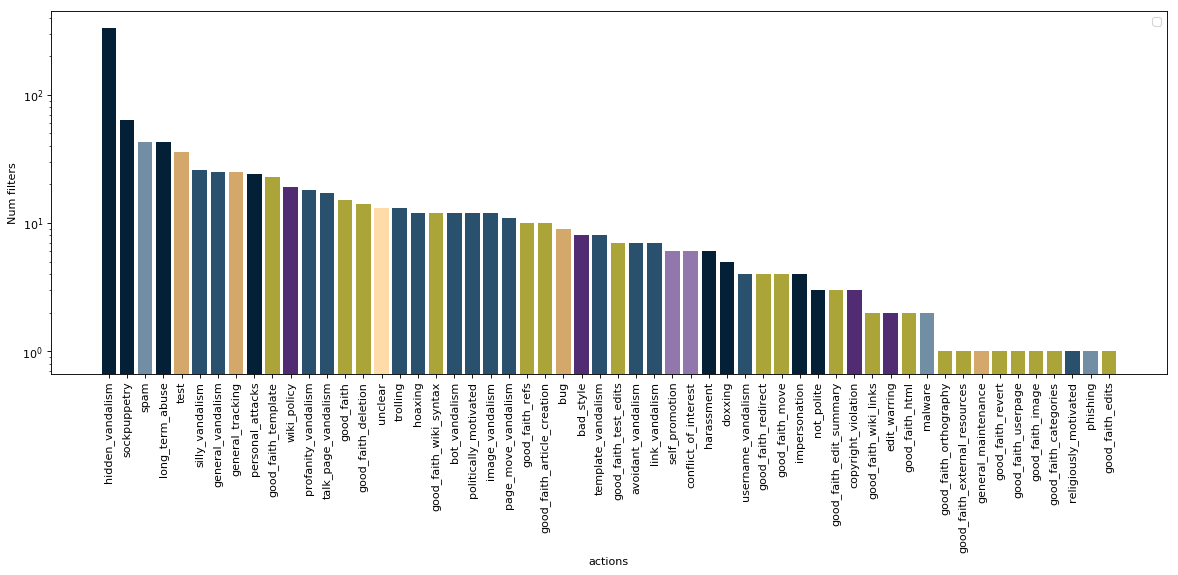
\includegraphics[width=0.9\columnwidth]{pics/manual-tags-distribution.png}
  \caption{Edit filters manual tag distribution}~\label{fig:manual-tags}
\end{figure}

%TODO discuss figure
\begin{comment}
* maybe just plot the parent categories and have a closer look at one of them exemplarily
* maybe merge parent categories and only work with ``vandalism'', ``good faith'' and ``maintenance'' (and ``unknown'')
\end{comment}


\subsection{What filters were implemented immediately after the launch + manual tags}
%TODO What were the first filters to be implemented immediately after the launch of the extension?
The extension was launched on March 17th, 2009.
Filter 1 is implemented in the late hours of that day.
Filters with IDs 1-80 (IDs are auto-incremented) were implemented the first 5 days after the extension was turned on (17-22.03.2009).
So, apparently the most urgent problems the initial edit filter managers perceived were:
page move vandalism (what Filter 1 initially targeted; it was later converted to a general test filter);
blanking articles (filter 3)
personal attacks (filter 9,11) and obscenities (12)
some concrete users/cases (hidden filters, e.g. 4,21) and sockpuppetry (16,17)

\subsection{Combine most active filters with manual tags}

\section{Fazit}


%TODO do something with this
\begin{comment}
Interestingly, there was a guideline somewhere stating that no trivial formatting mistakes should trip filters\cite{Wikipedia:EditFilterRequested}
%TODO (what exactly are trivial formatting mistakes? starting every paragraph with a small letter; or is this orthography and trivial formatting mistakes references only Wiki syntax? I think though they are similar in scale and impact)
I actually think, a bot fixing this would be more appropriate.
\end{comment}

\begin{comment}
## Open questions

If discerning motivation is difficult, and, we want to achieve different results, depending on the motivation, that lead us to the question whether filtering is the proper mechanism to deal with disruptive edits.

%TODO doesn't really seem related, maybe get rid of it altogether
    Well, on the other hand, I'd say there are filters that seem to be there in order to protect from malicious activity (the vandalism filters) and such that kind of enhance the MediaWiki functionality: by providing warning messages (with hopefully helpful feedback) or by tagging behaviours to be aggregated on dashboards for later examination
Vgl \cite{HalRied2012}
Bot taxonomy

Task area                           | Example
-----------------------------------------------------
Content
 injection                          | RamBot
 monitoring                         | SpellCheckerBot
 curating                           | Helpful Pixie Bot ("corrects ISBNs and other structural features of articles such as section capitalization")
                                    | interlanguage bots (deprecated bc of Wikidata?)
------------------------------------------------------
                                    |
Augment MediaWiki functionality     | AIV Helperbot "turns a simple page into a dynamic
priority-based discussion queue to support administrators in their work of identifying and
blocking vandal"                    | SineBot - signs and dates comments


------------------------------------------------------

Protection from malicious activity  | ClueBot_NG
                                    | XLinkBot


\end{comment}
